\documentclass[tikz]{standalone}
\usepackage{times}
\usepackage{amsmath}
\usepackage{txfonts}
\usepackage{xcolor}
\usepackage[utf8]{inputenc}
\usepackage{graphics}
\usepackage{pgfplots}
\usetikzlibrary{spy}
\usetikzlibrary{calc}
\usetikzlibrary{arrows.meta}
\usetikzlibrary{patterns}
\usetikzlibrary{pgfplots.fillbetween}
\usepackage{ifthen}
\begin{document}
	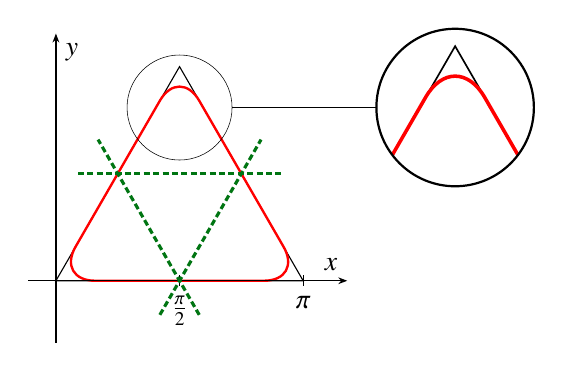
\begin{tikzpicture}[spy using outlines={circle, magnification=1.5, size=3cm, connect spies}]
		\definecolor{clrGreen}{RGB}{0, 117, 18}
		
		\def\sidelength{3.14}
		
		\pgfmathsetmacro{\triangleheight}{sqrt(3)/2*\sidelength}
		
		\draw[fill=white] (0,0) -- (\sidelength,0) -- (0.5*\sidelength, 	\triangleheight) -- cycle;
		
		\draw[red, line width=0.3mm, rounded corners=0.5cm] (0,0) -- 	(\sidelength,0) -- (0.5*\sidelength, \triangleheight) -- cycle;
		
		\draw[->,{line width=0.5pt},>={Stealth[scale=0.62]}] (-0.35,0) -- (3.7,0) node[above left] {$x$};
		\draw[->,{line width=0.5pt},>={Stealth[scale=0.62]}] (0,-0.785) -- (0,3.14) node[below right] {$y$};
		
		\foreach \x/\xlabel in {1.5708/$\frac{\pi}{2}$, 3.14159/$\pi$}
		\draw (\x,2pt) -- (\x,-2pt) node[below] {\xlabel};
		
		\draw[clrGreen, dashed, dash pattern=on 2.2pt off 1.2pt, dash phase=0.2pt, line width=0.4mm] (3.14156/4-0.5, 	\triangleheight/2) -- (0.75*\sidelength+0.5, \triangleheight/2);
		\draw[clrGreen, dashed, dash pattern=on 2.2pt off 1.2pt, dash phase=0.4pt, line width=0.4mm] (3.14156/4-0.25, 	\triangleheight/2+0.433) -- (0.5*\sidelength+0.25, 0-0.433);
		\draw[clrGreen, dashed, dash pattern=on 2.2pt off 1.2pt, dash phase=0pt, line width=0.4mm] (0.5*\sidelength-0.25, 0-0.433) 	-- (0.75*\sidelength+0.25, \triangleheight/2+0.433);
		\spy [size=2cm] on (1.57,2.2) in node [right] at ($(1.57,2)+(2.5,0.2)$);
	\end{tikzpicture}
\end{document}